\documentclass[12pt,a4]{article}
\pagestyle{plain}                           

% Use Report Template
\usepackage{temp/report_template}

% For appendix
\usepackage[toc,page]{appendix}

% For Better Tables
\usepackage{tabularx}

% For Fortran Code
\usepackage{listings}
\lstset{language=[90]Fortran,
  basicstyle=\ttfamily,
  keywordstyle=\bfseries,
  commentstyle=\itshape,
  morecomment=[l]{!\ },% Comment with only space after !
  showstringspaces=false,
  frame=topline
}

% For Subfiles
\usepackage{subfiles}

% Graphics Path
\graphicspath{{img/}{../img/}}

% Indent
\setlength\parindent{1 in}

\begin{document}
\title{Naive Tsunami Generation via Shallow Water Theory\\
\large  MATH484 Final Project Report}
\author{John Luke Lusty, Jonah Kopp, Clay Kramp, Lonny Cox-Lauf}
\date{April 12\textsuperscript{th}, 2018}

\begin{titlepage}
	\maketitle
    \begin{figure}[h]
        \centering
        \fbox{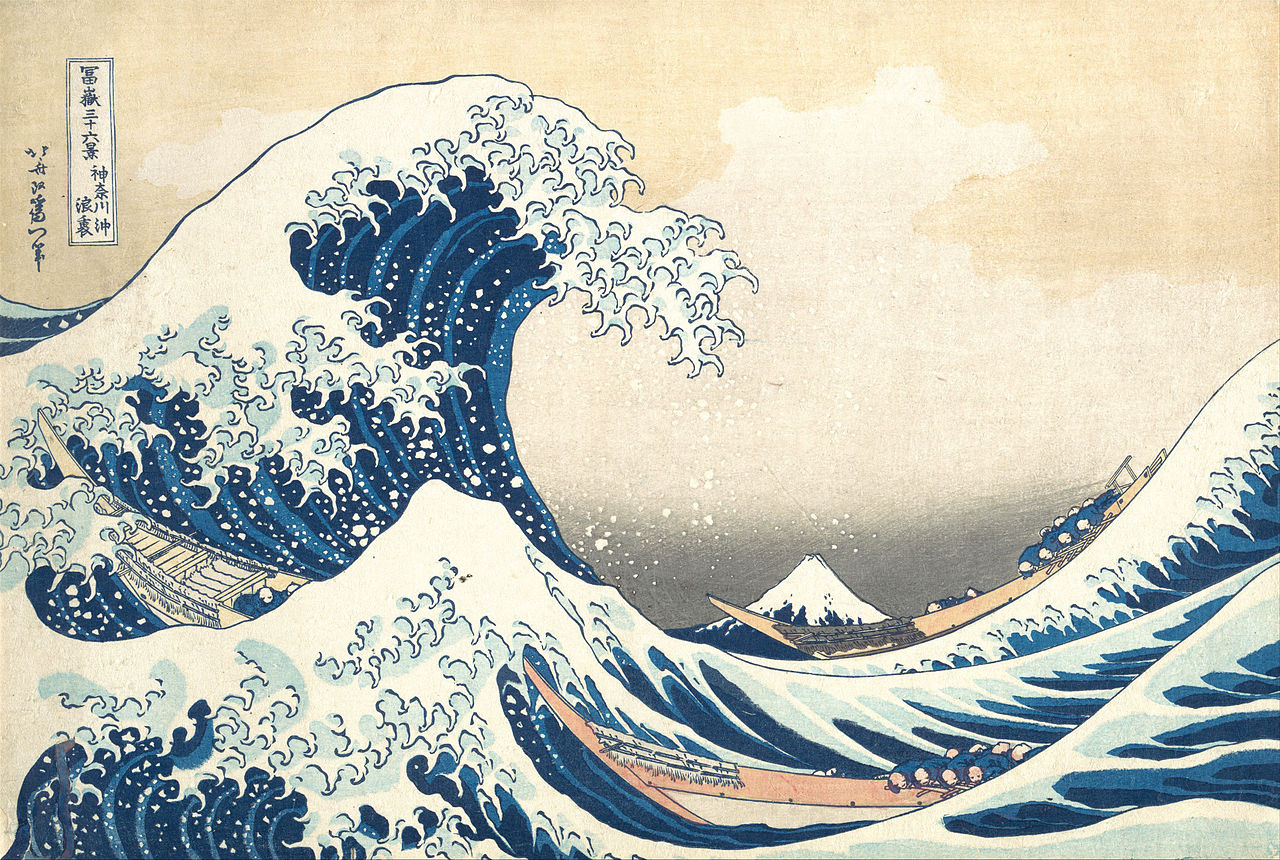
\includegraphics[width=\textwidth]{great_wave}}
        \caption*{\textit{"The Great Wave off Kanagawa"}, Katsushika Hokusai est. 1829}
    \end{figure}
\end{titlepage}
	
\tableofcontents
\pagebreak

% INTRODUCTION
\section{Introduction}
\subfile{sec/intro}

% SHALLOW-WATER THEORY
\section{Shallow-Water Theory}
\subfile{sec/shallow}

% CONSERVATIVE FORM
\section{The Conservative Form of a Hyperbolic Equation}
\subfile{sec/conserve}

% NUMERICAL METHODOLOGY
\section{Numerical Methodolgy}
\subfile{sec/numerics}

% APPLICATION
\section{Application: Fukushima Daiichi Nuclear Disaster}
\subfile{sec/app}

% BEZIER
\section{Interpolating Sea Floor: Fukushima Daiichi Nuclear Disaster}
\subfile{sec/bezier}

\appendix
\section{Derivation of The Shallow Water Equations}\label{a:deriv}
\colorbox{red}{Later.}
\section{The Leapfrog Method}
\subsection{Stability}
\colorbox{red}{Later.}
\subsection{Consistency}
\colorbox{red}{Later.}
\subsection{Convergence}
\colorbox{red}{Later.}

\begin{thebibliography}{1}
\bibitem{zirker}
Jack B Zirker.
\textit{The Science of Ocean Waves: Ripples, Tsunamis, and Stormy Seas}.
John Hopkins University Press, 22 October 2013. 
Accessed via Arthur Lakes Library at the Colorado School of Mines, March 31, 2018.
    
\bibitem{marghany}
Maged Marghany.
\textit{Simulation of Tsunami Impact on Sea Surface Salinity along Banda Aceh Coastal Waters, Indonesia}.
Advanced Geoscience Remote Sensing, Ch 3. Intech, 2014. Accessed via In Tech Open, March 31, 2018.
    
\bibitem{satake1}
Yuichiro Tanioka, Kenji Satake.
\textit{Tsunami generation by horizontal displacement of ocean bottom}.
Geophysical Research Letters, Vol 3, No 8, 15 April 1996. American Geophysical Union Publications. Accessed via Wiley Online Library, March 31, 2018.

\bibitem{salmon}
Rick Salmon.
\textit{Introduction to Ocean Waves}.
Scripps Institution of Oceanography, University of California, San Diego, 7 December 2015. Accessed via Rick Salmon's website via http://pordlabs.ucsd.edu/rsalmon/, March 31, 2018.

\bibitem{rezzolla}
Luciano Rezzolla.
\textit{Lecture Notes on Numerical Methods for the Solution of Hyperbolic Partial Differential Equations}.
SISSA, International School of Advanced Studies, Trieste, Italy, 2 August 20015. Accessed via Luciano Rezzolla's website via http://www.sissa.it/~rezzolla, March 31, 2018.

\end{thebibliography}
	
\end{document}
